\section{Methodology and Implementation}
% What were the methods used?
% How was the problem designed?
% Driving concepts
% Equations
% Figures

A modular, agent-based simulator is an ideal approach for solving complex, coupled,
physics-dependent supply chain problems involving material routing, facility
deployment, and regional and institutional hierarchies. Additionally, the choice to 
build \Cyclus on open source libraries in modern programming languages enables 
both remote and mutiprocess execution on a number of platforms.

\subsection{Cluster-Ready Software}

Many fuel cycle simulators rely on \gls{COTS} and Windows-only software that limits 
performance on resource computing infrastructures. This limitation severely 
increases the wall-clock time necessary to conduct parameterized sensitivity 
analyses and other multi-simulation studies. 

\Cyclus, on the other hand, is primarily written in \texttt{C++} and relies on 
libraries supported by Linux and UNIX (including Ubuntu and OSX) platforms. 
Furthermore, the core infrastructure and related archetypes are free and 
open source, BSD-3-clause licsened. No part of \Cyclus is proprietary or based 
on \gls{COTS}, Windows-based software. It can be easily deployed 
on large computer systems, such as \gls{HTC} systems.

Cyclopts (\TODO{cite}), a proof of principle design and implementation of such a
system, uses UW-Madison's HTCondor \gls{HTC} infrastructure to perform sensitivity
studies on \Cyclus' resource exchange optimization solvers. To date, it has been
used run over $10^4$ jobs, or (\TODO{compute time}) total compute hours, using
the \Cyclus library via its resource exchange \gls{API}.
The \gls{HTC} infrastructure has also been utilized to run and collect
information from full \Cyclus simulations running in parallel on $10^3$
machines reliably for order $10^5$ simulations.


\subsection{Framework Structure}
% (OO, cpp, xml, backends, inheritances, mixins, generic apis, etc.)

\acrlong{ABM} is inherently object-oriented. Since agents represent 
discrete, independently acting objects, object-orientation is the natural 
paradigm in which to conduct \gls{ABM}.

The core of the \Cyclus simulator creates a set of key classes on which agent 
plug-ins 
are based. In addition, a set of key tools are also provided to enrich the 
\gls{API} and supply a robust suite of behaviors for the developer.


\begin{figure}[htbp!]
\begin{center}
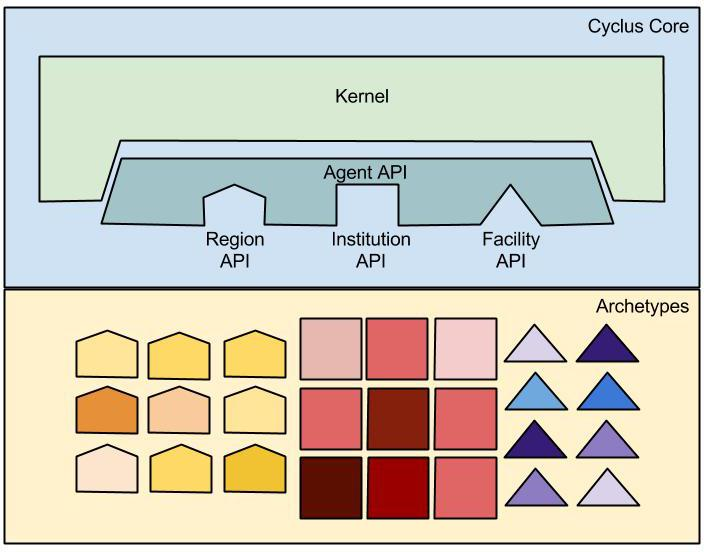
\includegraphics[width=\textwidth]{./images/framework}
\end{center}
\caption{The \Cyclus core provides \gls{API}s that abstract away the details in 
the kernel and allow the archetypes to be loaded into the simulation in a modular 
fashion.}
\label{fig:framework}
\end{figure}

Agent plug-ins utilize the generic core \gls{API} to interact with one another.  For 
example, agents rely on the dynamic loading and paradigm for clean plug-in 
behavior at the start of the simulation. They also use the resource exchange 
paradigm \gls{API} for trading resources with one another. 


\subsection{Dynamically Loadable Libraries}
% (diagram)

A key innovation in \Cyclus is implementing this generic \gls{API} and modular 
architecture into a suite of dynamically loadable plug-in libraries.  Though 
common in modern software architecture, such a plug-in pattern has 
previously not been implemented in nuclear fuel cycle simulators in the 
literature.  In \Cyclus, this implementation maximizes the potential of the clean, 
object-oriented \gls{API} and modern build system already described.

Dynamically loadable libraries are the primary mechanism for extending \Cyclus' capability. 
This approach provides encapsulation: the core of the code operates
completely independently from the individual plug-in libraries. Thus, any
customization or extension is implemented only in the loadable
library. 

This approach encourages efficient, targeted contribution to the ecosystem of 
archetype libraries.  The 
scientist-developer can focus on generating an archetype model within their
sphere of expertise, while relying on the contributions of others to furnish
the other technologies in the simulation.  This strategy also allows individual developers to
explore different levels of complexity within their archetypes, including
wrapping other simulation tools as loadable libraries within the \Cyclus
framework.

A secondary benefit is the ability for
contributors to choose different distribution and licensing strategies
for their contributions. By allowing models to have varied
availability, the security concerns of developers can be
assuaged (See Figure \ref{fig:modifiedopen}).

\begin{figure}[htbp!]
\begin{center}
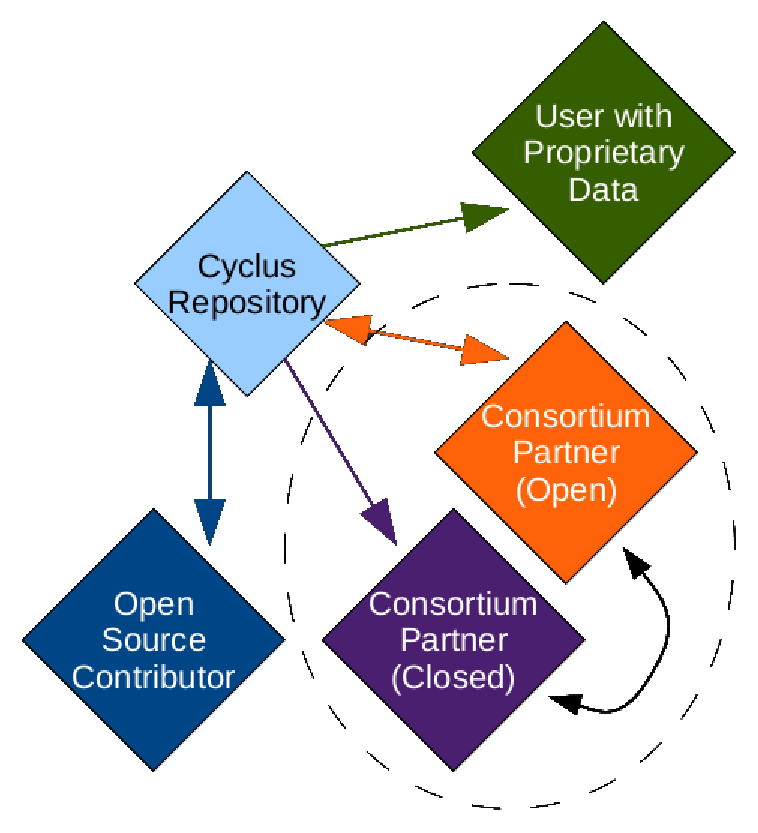
\includegraphics{./images/modifiedopen.eps}
\end{center}
\caption{The \Cyclus framework enables fully open, partially open, and fully
closed collaborations\cite{carlsen_cyclus_2014}.}
\label{fig:modifiedopen}
\end{figure}

In particular, since the clean plug-in architecture loads libraries without any
modifications to the \Cyclus kernel, closed-source archetypes can be used with
the simulator alongside open source archetypes. This architecture
allows closed-source libraries (e.g., those representing sensitive nuclear
processes and subject to export control) to be developed and licensed privately.

This last benefit of dynamically loadable libraries addresses
another goal of \Cyclus: ubiquity amongst its potential user base. By
engineering \Cyclus to easily handle varying levels of complexity, a single
simulation engine can be used by both users interested in big-picture policy
questions as well as users focused on more detailed, technical
analyses. They merely choose their preferred level of fidelity from the 
available libraries. 

\subsection{Agent Interchangability}\label{sec:interchangeability}

Due to this plug-in architecture,
implementations of actors in a given simulation can be easily
interchanged. Critically, this novel functionality enables the comparison
between agent implementations. For example, a low-physics-fidelity
implementation of a reactor can be compared to an implementation with higher
physics fidelity, allowing an analyst to discern the effect of reactor physical
fidelity on a given fuel cycle. 

Interchangability is accomplished by providing \glspl{API} that define agent-to-agent
interaction and agent-to-environment interaction, primarily through the
\Class{Agent} and \Class{Trader} interfaces. Figure \ref{fig:agent_uml} shows 
the ``inheritance'' structure of the \Class{Agent} class in a \gls{UML} diagram 
format. It shows how the \Class{Agent} interface
provides a notion of parent-child hierarchichal relationship, where parents can
choose to \textit{build} child agents and \textit{decommission} child
agents. For the archetype developer, this interface provides enormous power, 
very simply. The \gls{API} exposes \Class{Agent} helpful functionality for 
interacting with the \Cyclus simulation kernel while abstracting away unnecessary 
detail.

\begin{figure}[htbp!]
\begin{center}
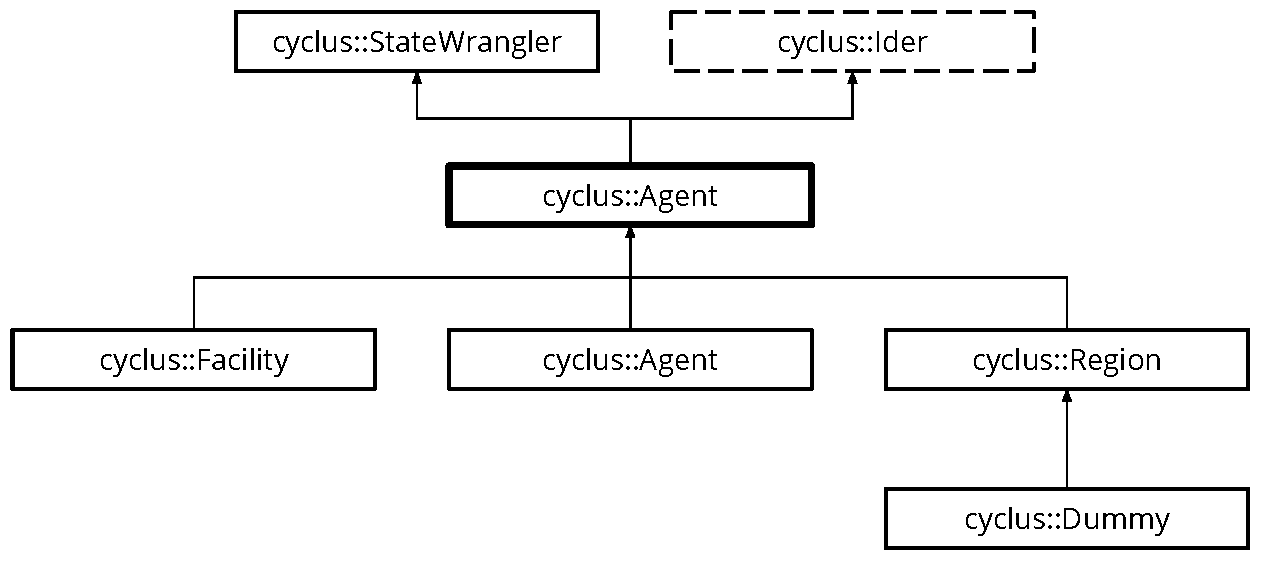
\includegraphics[width=0.5\textwidth]{./images/agent_uml}
\end{center}
\caption{The inheritance in \Cyclus classes, such as the \Class{Agent}, 
\Class{Facility}, \Class{Institution}, and \Class{Region} classes abstract away 
unneccesary details while exposing powerful functionality. In the above 
example, the \Class{Dummy} archetype simply inherits from \Class{Region} in 
order to become a bonified Region-type \Class{Agent}.}
\label{fig:agent_uml}
\end{figure}

In a similar fashion, the \Class{Trader} interface allows agent-to-agent interaction through the
trading of \Class{Resource}s. Usable archetypes in a \Cyclus simulation must
implement the \Class{Agent} interface and may optionally implement the
\Class{Trader} interface. For example, a \Class{Region} implements only the
\Class{Agent} interface, whereas a \Class{Facility} implements both the
\Class{Agent} and \Class{Trader} interface, allowing any \Class{Facility} to
trade with another \Class{Facility}.

In this way, a researcher can directly compare two different reactor modeling 
implementations (perhaps \Class{DetailedReactor} and \Class{SimpleReactor}) 
simply by exchanging the two corresponding archetypes. That is, two reactor 
archetypes both inheriting from the \Class{Facility} class are indistinguishable 
from a simulation perspective. Two simulations, one using 
\Class{DetailedReactor} and the other using \Class{SimpleReactor} can therefore 
be compared directly to determine the impact of using one or the other model.
This can be done with any agent type, where agents can be ``Regions,'' 
``Institutions,'' or ``Facilities.''

\subsection{Regions, Institutions, and Facilities}

\Cyclus provides a novel representation of entities in the nuclear fuel cycle 
which mimics the reality in international nuclear power production
including facilities, institutions managing those facilities, and regions. While
some simulators (\TODO{cite DESAE}) have provided a notion of static regional
effects, \Cyclus allows for both regions and institutions to be first-class
actors in simulated fuel cycles.

The fundamental interactions for each entity are implemented in a corresponding
archetype class in \Cyclus, i.e., the \Class{Region} class, \Class{Institution}
class, and \Class{Facility} class. Archetype developers can then build on the
provided functionality by inheriting from the appropriate class.

\Cyclus implements a \gls{RIF} relationship through the
parent-child hierarchy described in \S \ref{sec:interchangeability}, where
regions are the parents of institutions which are, in turn, the parents of
facilities. In other words, \gls{RIF} hierarchies form a directed acyclic graph (DAG),
with regions as root nodes and facilities as leaf nodes.

Two primary consequences arise from this structure. First, institutions are
responsible for building and decommissioning facilities, so advanced
logic regarding building and decommissioning can be obtained by subclassing the
\Class{Institution} interface. Second, the \Class{Facility} class implemenets the
\Class{Trader} interface, and thus institutions and regions can
adjust the resource flow preferences of their managed facilities, respectively. Importantly,
this novel capability allows for the modeling of preferential regional trading
of resources (e.g., tariffs) as well as preferential institutional trading
(e.g., long-term contracts).

Although concept of the \gls{RIF} hierarchy is provided, the \Cyclus kernel is
designed to handle hierarchies of arbitrary depth.
A simulation can proceed without regions and institutions (i.e.,  only facilities)
or with archetypes that are the parents of regions.  By
convention, institutions are mainly responsible for facility deployment, but
any archetype can have access to \Cyclus' agent deployment mechanism.  It is straightforward
to implement agents that deploy copies of themselves or schedule their
own decommissioning.  Because regions, institutions, and facilities are all
agents, they can all be implemented to exercise the full set of features
offered by the \Cyclus kernel.

\subsection{Resources and Materials}
% Resources, Materials (note isotope tracking, decay behavior)

\TODO{add blurb about discrete agent/facility tracking.}

In \Cyclus, agents can transfer discrete resource objects between each other.
Cyclus supports two types of resources:

\begin{itemize}

  \item Materials: These represent typical nuclear materials with
      nuclide-based compositions.

  \item Products: These can represent any user-defined measure - e.g. carbon
      credits, build permits, employees, etc.

\end{itemize}

All operations performed on resource objects (splitting, combining,
decay, etc.) are tracked in detail.  This information includes the creating
agent for when resources are newly created and introduced into the simulation.
The parentage of each resource is also tracked. This makes it possible to
follow the history of discrete resource objects as they are transferred
between agents, powerfully impacting the ability to model 
non-proliferation-related simulation goals. 

The \Cyclus kernel has built-in experimental support for decay calculations.
Materials ``remember'' the time since their last decay and agents are free to
invoke the decay function on them as desired to decay them to the current
simulation time. \Cyclus can currently operate in 2 decay modes with 2 other
modes likely to be added in future releases:

\begin{itemize}

    \item "manual" (currently implemented) is the default mode just described
        where agents decay materials as needed.

    \item "never" (currently implemented) globally turns off all decay.
        Materials' decay function does nothing.

    \item "periodic" (future) automatically decays all materials in a
        simulation with some fixed frequency.

    \item "lazy" (future) decays any material whenever its composition is
        viewed (e.g. when an agent queries information about a material's
        $^{239}$Pu content).

\end{itemize}

In order to avoid excess decay calculations, when a material's decay function
is invoked, the material compares the decay constants of its nuclides with
the time delta for the current
decay operation.  If all the decay constants are not significant, no decay
calculation is performed and the material remains unchanged.  This error does
not accumulate because the next time the material's decay function is invoked,
the time delta will be larger. \TODO{want more detail on this decay shortcut?}
\TODO{describe decay algorithm and how it might be improved}.

\Cyclus has no notion of "tracked" nuclides.  In \Cyclus, a  material's
composition represents an arbitrarily large list (potentially thousands) of
nuclides.  Agents are free to treat nuclides present in materials any way they
please - including ignoring them.  It is the responsibility of archetype
developers to choose how to handle potentially full-fidelity compositions.

In large simulations there may be many material objects changing frequently, on 
the day or month timescale.
Material decay can also contribute significantly to such changes.  In order to
help avoid unnecessary runtime performance and database space impacts,
compositions in \Cyclus have some special features, such as immutability.
Immutable compositions allow multiple material objects to all hold
references to the same composition object safely.  When operations are
performed on a material that do not alter the composition, any new resulting
materials hold a reference to the same, originating composition object.
Although the decay operation generates a new, separate composition (preserving
immutability), a reference to the new composition is placed in a cache shared
by the new and originating compositions. The next time the originating
composition is decayed, this cache will be checked for a prior calculation
with the same cumulative decay time.  If one exists, the cached composition is
used.  This cache is shared by all compositions that transitively come from
the same origin.  Composition immutability in concert with decay history
caching help eliminate many redundant decay calculations in addition to
reducing the total number of composition objects.  Since each composition
object is only recorded in the database once, significant space savings also
occurs. \TODO{do we want a diagram helping show this composition caching?}

\subsection{Toolkit}

In addition to the core functionality of the \Cyclus kernel, which is focused on
the minimal set of capabilities needed to implement an agent-based simulation
with dynamic resource exchange, a toolkit is provided that assists developers
and users with related simulation and nuclear engineering tasks. The toolkit is
an actively developed module of \Cyclus, with a primary forward-looking
focus on supporting interesting \textit{in situ} (i.e., in simulation) and
\textit{ex situ} (i.e., post-processing) metric analysis tools. 

\subsubsection{Simulation Tools}

A series of utility classes are provided to support demand-constrained agent
(e.g., facility) deployment. Symbolic function representations of linear,
exponential, and piecewise functions are supported via the
\Class{SymbFunctionFactory} class. Such functions are used with other toolkit
classes to determine commodity demand (e.g., power demand) from user input. Four
mixin classes provide the basis for in-simulation deployment determination:
\Class{CommodityProducer}, \Class{CommodityProducerManager}, \Class{Builder},
and \Class{BuildingManager}. The \Class{CommodityProducer} class provides an
interface for querying the \textit{prototypes} that have some nameplate
capacity to produce a given commdity, and the \Class{CommodityProducerManager}
provides an interface for registering \Class{CommodityProducer}s and querying
the current capacity (supply) of a commodity. The \Class{Builder} class provides
an interface for querying which prototypes can be built and interacts with the
\Class{BuildingManager}, which orders prototypes to be built. The
\Class{BuildingManager} uses a simple minimum cost algorithm to determine how
many of each prototype, $y_i$, to build given a demand, $\Phi$, capacities,
$\phi_i$, and costs, $c_i$.

\begin{equation}
\begin{aligned}
 \min & \sum_{i=1}^{N}c_i y_i \\
 s.t. & \sum_{i=1}^{N}\phi_i y_i \ge \Phi \\
      & n_i \in [0,\infty) \:\: \forall i \in I, \:\: y_i \:\: \text{integer} 
\end{aligned}
\end{equation}

\subsubsection{Nuclear Engineering Tools}

The \Cyclus toolkit provides two useful modules for querying \Class{Material}
objects regarding physical parameters. First, the \Class{MatQuery} module
provides a basic querying \gls{API}, including the atom and mass fractions of
nuclides, the number of moles of a nuclide in a material, and also the amount of
aggregate nuclides, i.e., a \Class{Composition}, in a material. The
\Class{enrichment} module provides an \gls{API} for determining enrichment-related
parameters of a material, including the separative work units (SWU) and natural
uranium required to enrich a material provided knowledge of feed, product, and tails
assays.

\subsubsection{Toolkit Extensions}

In addition to those that already exist, tools and computational patterns will 
emerge from the archetypes that are developed within the community of 
developers. As those tools gain adoption between projects and demonstrate their 
utility to the developer community, they will be considered for screening and 
adoption into the kernel as toolkit extensions. Likely extensions include:

\begin{itemize}
\item fuel cycle metrics calculators
\item supportive data tables
\item policy models
\item economic models
\item etc.
\end{itemize}

\subsection{Cycamore}
% base modules

\Cycamore \cite{carlsen_cycamore_2014}, the \Cyclus additional modules 
repository, provides a fundamental set of agent archetypes for basic simulation 
functionality within \Cyclus.  Since the \Cyclus framework relies on external 
archetypes to represent the agents within a simulation, \Cycamore provides the 
basic archetypes a new user needs to get started running simple simulations.  
These archetypes support a minimal set of fuel cycle simulation goals and 
provide, by example, a guide to new developers who would seek to contribute 
their own archetypes outside of \Cycamore.

As of version 1.0, \Cycamore contains four facility archetypes, one region 
archetype, and two institution archetypes. Short descriptions of those 
functions can be found in Table \ref{tab:cycamore}.


\begin{table}[h]
\centering
\begin{tabularx}{\textwidth}{|r|l|X|}
\hline
\textbf{Agent Type} & \textbf{Archetype} & \textbf{Functionality} \\
\hline
Facility & BatchReactor & A reactor model that handles batch refuelling, based on pre-determined recipes of compositions. \\
Facility & Source & This facility generates material of the composition and commodity type specified as input.  \\
Facility & Sink & This facility is capable of accepting a finite or infinite quantity of some commodity produced in the simulation. \\
Facility & EnrichmentFacility & This facility enriches uranium at a specified capacity. \\
Institution & ManagerInst & The manager institution manages production of commodiites among its facilities by building new necessary ones. \\
Institution & DeployInst &  This institution deploys specific facilities as defined explicitly in the input file. \\
Region & GrowthRegion & This region determines whether there is a need to meet a certain capacity (as defined via input) at each time step. \\
\hline
\end{tabularx}
\caption{The Archetypes in \Cycamore seek to cover a large range of simple simulation use cases.}
\label{tab:cycamore}
\end{table}

As future contributions are vetted, the capabilities in \Cycamore may grow. 
However, the current \Cycamore release provides only 
basic functionality, enabling simple fuel cycle analyses. 
\Cycamore is provided so that users can get started quickly with simple 
analyses.

Figure \ref{fig:simplesim} shows an example of a simple, once-through fuel cycle 
that can be generated with \Cycamore and \Cyclus alone.

\begin{figure}[htbp!]
\begin{center}
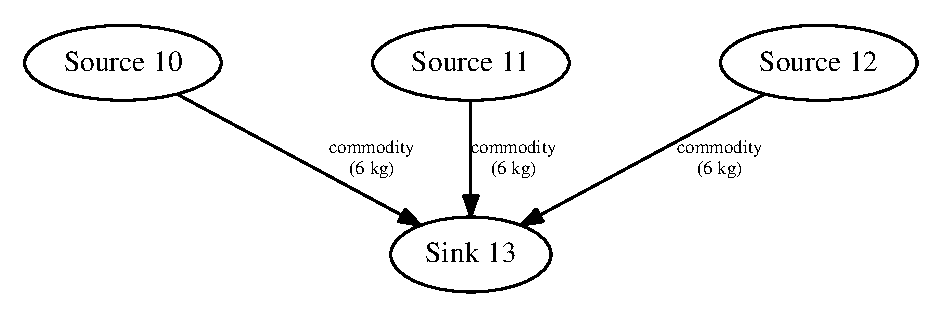
\includegraphics{./images/simplesim}
\end{center}
\caption{Material flows through a simple dynamic simulation created with only the simplest \Cycamore archetypes, \Class{Sink} and \Class{Source}.}
\label{fig:simplesim}
\end{figure}
